
%% Harvard Physics Project
%% Test Booklet 2: Motions in the Heavens
%%--------------------------------------------------


%% Test Booklet 2 contains 70 questions


%% Test A
%%--------------------
\element{project}{
\begin{question}{testA-Q01}
    To ancient observers, the principal difference between
        the planets and the stars was that the planets appeared:
    \begin{choices}
        \wrongchoice{brighter.}
        \wrongchoice{more like the earth.}
      \correctchoice{to wander among the other stars,}
        \wrongchoice{closer to the earth.}
        \wrongchoice{to travel around the sun.}
    \end{choices}
\end{question}
}

\element{project}{
\begin{question}{testA-Q02}
    Which of the following statements must be part of any heliocentric theory?
    \begin{choices}
      \correctchoice{The planets revolve around the sun,}
        \wrongchoice{The sun is a sphere.}
        \wrongchoice{The earth is a sphere.}
        \wrongchoice{The planets revolve around the earth,}
        \wrongchoice{The earth turns on its axis.}
    \end{choices}
\end{question}
}

\newcommand{\FoneFtwo}{
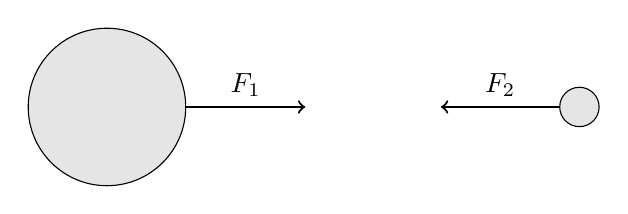
\begin{tikzpicture}
    %% Objects
    \node[draw,fill=white!90!black,circle,minimum size=2cm] (A) at (-3,0) {};
    \node[draw,fill=white!90!black,circle,minimum size=0.5cm] (B) at (3,0) {};
    %% Forces
    \draw[thick,->] (A.east) -- ++(0:1.51cm) node[pos=0.5,anchor=south] {$F_1$};
    \draw[thick,->] (B.west) -- ++(180:1.5cm) node[pos=0.5,anchor=south] {$F_2$};
\end{tikzpicture}
}

\element{project}{
\begin{question}{testA-Q03}
    If $F_1$ is the magnitude of the force exerted on the
        sun by the earth and $F_2$ is the magnitude of the
        force exerted on the earth by the sun, then:
    \begin{center}
        \FoneFtwo
    \end{center}
    \begin{choices}
        \wrongchoice{$F_1$ is much greater than $F_2$.}
        \wrongchoice{$F_1$ is slightly greater than $F_2$.}
      \correctchoice{$F_1$ is equal to $F_2$.}
        \wrongchoice{$F_1$ is slightly less than $F_2$}
        \wrongchoice{$F_1$ is much less than $F_2$}
    \end{choices}
\end{question}
}

\element{project}{
\begin{question}{testA-Q04}
    Which one of the following men is famous for the decision
        to abandon Plato's association of heavenly bodies with
        ``uniform motion in perfect circles''?
    \begin{multicols}{2}
    \begin{choices}
        \wrongchoice{Aristotle}
        \wrongchoice{Copernicus}
      \correctchoice{Kepler}
        \wrongchoice{Galileo}
        \wrongchoice{Tycho Brahe}
    \end{choices}
    \end{multicols}
\end{question}
}

\element{project}{
\begin{question}{testA-Q05}
    Galileo gathered a great deal of evidence which was
        at odds with the medieval view of the universe.
    \emph{All except one} of the following are examples of this evidence.
    Which is the exception?
    \begin{choices}
        %% Supernova
        \wrongchoice{the discovery of a new star in 1604}
        %% Deviation from perfect sphere
        \wrongchoice{the rough appearance of the moon's surface}
        %% Supported Copernican system
        \wrongchoice{the motion of four luminous objects around Jupiter}
        %% Supported Copernican system
        \wrongchoice{the moon-like phases of planet Venus}
      \correctchoice{the wanderings of the planets among the stars}
    \end{choices}
\end{question}
}

\element{project}{
\begin{question}{testA-Q06}
    Two sacks of marbles are hung one meter apart.
    Which of the following would approximately double the
        gravitational force that one sack of marbles exerts on the other sack?
    \begin{choices}
      \correctchoice{Double the number of marbles in one sack.}
        \wrongchoice{Double the number of marbles in both sacks.}
        \wrongchoice{Move them closer, to one-half the separation.}
        \wrongchoice{Move them further apart, to twice the separation.}
        \wrongchoice{Move them further apart, to four times the separation.}
    \end{choices}
\end{question}
}

\element{project}{
\begin{question}{testA-Q07}
    \emph{All except one} of the following statements are acceptable.
    Which is the exception?
    \begin{choices}
        \wrongchoice{The earth is moving fastest when closest to the sun. }
        \wrongchoice{The path of the earth lies in a plane which passes through the sun. }
        \wrongchoice{A line drawn from the sun to the earth sweeps over the same area from March 21 to March 23 as it does from December 21 to December 23. }
      \correctchoice{The sun is at the exact center of the earth's path.}
    \end{choices}
\end{question}
}

\element{project}{
\begin{question}{testA-Q08}
    Assume that the earth suddenly shrank to one-half its original diameter,
        but that its mass remained unchanged.
    Under these circumstances,
        the weight of a person standing on its surface would be:
    \begin{choices}
      \correctchoice{four times as great.}
        \wrongchoice{twice as great.}
        \wrongchoice{the same.}
        \wrongchoice{one-half as great.}
        \wrongchoice{one-fourth as great.}
    \end{choices}
\end{question}
}

\element{project}{
\begin{question}{testA-Q09}
    A friend tells you the earth is fixed in space and that the sun revolves about it.
    Which one of the following facts contradicts his hypothesis?
    \begin{choices}
        %% NOTE: these were all well known and explained by both models
        \wrongchoice{Each day the sun rises in the east and sets in the west.}
        \wrongchoice{During the night the stars appear to move.}
        \wrongchoice{The sun makes one complete trip among the stars in one year.}
        \wrongchoice{Eclipses of the sun sometimes occur.}
      \correctchoice{none of the provided}
    \end{choices}
\end{question}
}

\element{project}{
\begin{question}{testA-Q10}
    Which one of the following was an important factor that worked
        against the acceptance of Copernicus' heliocentric solar
        system hypothesis in the sixteenth century?
    \begin{choices}
        \wrongchoice{When Venus was observed through a telescope, phases were seen.}
      \correctchoice{Stellar parallax had never been observed.}
        \wrongchoice{The calendar failed to keep pace with the seasons.}
        \wrongchoice{Galileo observed four satellites moving around Jupiter.}
        \wrongchoice{Venus had never been observed more than \ang{48} from the sun.}
    \end{choices}
\end{question}
}

\element{project}{
\begin{question}{testA-Q11}
    \emph{All except one} of the following were among
        Tycho Brahe's contributions to astronomy.
    Which one is the \emph{exception}?
    \begin{choices}
        \wrongchoice{He established an astronomical observatory.}
      \correctchoice{He proposed an inverse square law of attraction for the solar system.}
        \wrongchoice{He developed a theory of the solar system.}
        \wrongchoice{He determined the limits of accuracy of his instruments.}
        \wrongchoice{He made very accurate observations of the positions of the heavenly bodies.}
    \end{choices}
\end{question}
}

\newcommand{\testAQTwelve}{
\begin{tabulary}{\columnwidth}{LLL}
    \multicolumn{1}{c}{Planet} &
    \multicolumn{1}{c}{Orbital Period} &
    \multicolumn{1}{c}{Mass} \\
    \midrule
    Alpha   & 14 earth years    & 10 earth masses \\
    Beta    & 188 earth years   & 17 earth masses \\
    Gamma   & 50 earth years    & $\frac{1}{2}$ earth mass \\
\end{tabulary}
}

\element{project}{
\begin{question}{testA-Q12}
    Assume that the following measurements were made on three planets revolving about a star.
    (Planets listed in order of discovery)
    \begin{center}
        \testAQTwelve
    \end{center}
    On the basis of Kepler's laws of planetary motion,
        these planets could be arranged in order of their
        increasing distance from the star.
    If the planets were listed in sequence,
        starting with the planet nearest the star,
        they would be arranged
    \begin{choices}
        \wrongchoice{Alpha, Beta, Gamma.}
        \wrongchoice{Beta, Gamma, Alpha.}
        \wrongchoice{Gamma, Alpha, Beta.}
        \wrongchoice{Beta, Alpha, Gamma.}
      \correctchoice{Alpha, Gamma, Beta.}
    \end{choices}
\end{question}
}

\element{project}{
\begin{question}{testA-Q13}
    The following men made significant contributions to our
        present understanding of planetary motion:
    \begin{enumerate}
        \itemsep=0pt
        \item Copernicus
        \item Newton
        \item Kepler
    \end{enumerate}
    If the names of these men were arranged in the order
        of their contributions starting with the earliest first,
        they would be:
    \begin{multicols}{3}
    \begin{choices}
        \wrongchoice{1, 2, 3}
        \wrongchoice{2, 3, 1}
        \wrongchoice{3, 1, 2}
      \correctchoice{1, 3, 2}
        \wrongchoice{2, 1, 3}
    \end{choices}
    \end{multicols}
\end{question}
}

\element{project}{
\begin{question}{testA-Q14}
    Time-exposure photographs of stars show arcs of circles.
    An astronomer who believed the Ptolemaic theory of
        planetary motion would explain that these arcs result from:
    \begin{choices}
        \wrongchoice{the rotation of the earth on its axis.}
        \wrongchoice{stellar parallax.}
        \wrongchoice{retrograde motion.}
        \wrongchoice{the inclination of the earth's axis.}
      \correctchoice{the rotation of the starry sphere.}
    \end{choices}
\end{question}
}

\element{project}{
\begin{question}{testA-Q15}
    Which one of the following is evidence that supports the
        universality of Newton's law of gravitation?
    \begin{choices}
      \correctchoice{Pairs of stars have been observed that move around each other in accordance with Kepler's laws.}
        \wrongchoice{A few stars have moved from the positions given for them in Ptolemy's catalogue of stars.}
        \wrongchoice{Stellar parallax has been observed for several thousand stars.}
        \wrongchoice{A calendar reform was needed in the sixteenth century to keep months and seasons in agreement.}
    \end{choices}
\end{question}
}


%% Test B
%%--------------------
\element{project}{
\begin{question}{testB-Q01}
    In its orbit, the earth travels:
    \begin{choices}
      \correctchoice{fastest when it is nearest the sun.}
        \wrongchoice{fastest at night.}
        \wrongchoice{fastest around the time of the new moon,}
        \wrongchoice{with constant speed.}
        \wrongchoice{zero speed, since the earth is stationary.}
    \end{choices}
\end{question}
}

\element{project}{
\begin{question}{testB-Q02}
    %Select answers to questions 2 and 3 from the following list.
    He tried to relate planetary distances to the
        five regular geometric solids.
    \begin{multicols}{2}
    \begin{choices}
        \wrongchoice{Ptolemy}
        %% NOTE: https://en.wikipedia.org/wiki/Platonic_solid
      \correctchoice{Kepler}
        \wrongchoice{Copernicus}
        \wrongchoice{Tycho Brahe}
        \wrongchoice{Galileo}
    \end{choices}
    \end{multicols}
\end{question}
}

\element{project}{
\begin{question}{testB-Q03}
    %Select answers to questions 2 and 3 from the following list.
    He developed a model of the solar system in which the
        planets revolved around the sun but the earth remained motionless.
    \begin{multicols}{2}
    \begin{choices}
      \correctchoice{Ptolemy}
        \wrongchoice{Kepler}
        \wrongchoice{Copernicus}
        \wrongchoice{Tycho Brahe}
        \wrongchoice{Galileo}
    \end{choices}
    \end{multicols}
\end{question}
}

\element{project}{
\begin{question}{testB-Q04}
    \emph{All except one} of the following are characteristics
        of geocentric models of the solar system.
    Which one is the \emph{exception}?
    \begin{choices}
        \wrongchoice{The earth is at or near the center of the solar system.}
        \wrongchoice{The stars are at the greatest distance from the earth.}
        \wrongchoice{The sun moves daily around the earth.}
      \correctchoice{The moon's motion is tied to the motion of the sun.}
        \wrongchoice{The stars move daily around the earth.}
    \end{choices}
\end{question}
}

\element{project}{
\begin{question}{testB-Q05}
    Kepler's three laws of planetary motion were:
    \begin{choices}
      \correctchoice{almost self-evident from Tycho Brahe's data of Mars' orbit.}
        \wrongchoice{little used in Newton's development of a general law of universal gravitation.}
        \wrongchoice{developed only after Kepler took imaginative steps from the available data.}
        \wrongchoice{widely discussed early in the seventeenth century.}
        \wrongchoice{used by Copernicus in deriving his heliocentric hypothesis.}
    \end{choices}
\end{question}
}

\element{project}{
\begin{question}{testB-Q06}
    Tycho Brahe's most important contribution to science was:
    \begin{choices}
      \correctchoice{the accurate observation of the positions of the stars and planets.}
        \wrongchoice{the discovery of a new star that changed its brightness.}
        \wrongchoice{the discovery of elliptical orbits.}
        \wrongchoice{his theory of planetary motions.}
    \end{choices}
\end{question}
}

\element{project}{
\begin{question}{testB-Q07}
    Galileo accumulated a great deal of evidence which was
        inconsistent with the medieval view of the universe.
    \emph{All except one} of the following are examples of this evidence.
    Which is the exception?
    \begin{choices}
        \wrongchoice{the discovery of a new star in 1604}
        \wrongchoice{the rough appearance of the moon's surface}
        \wrongchoice{the motion of four luminous objects around Jupiter}
        \wrongchoice{the moon-like phases of planet Venus}
      \correctchoice{the wanderings of the planets among the stars}
    \end{choices}
\end{question}
}

\element{project}{
\begin{question}{testB-Q08}
    A satellite with a television camera is placed in an orbit
        \SI{24 000}{\mile} above the earth so that it remains
        exactly above the same point on earth at all times,
        with its camera pointed toward the earth.
    As seen from the sun the orbit of the satellite is:
    \begin{choices}
        %% NOTE: https://en.wikipedia.org/wiki/Deferent_and_epicycle
        \wrongchoice{an ellipse with the sun at one focus.}
        \wrongchoice{an epicycle with its center on the orbit of the sun.}
      \correctchoice{an epicycle with its center on the orbit of the earth.}
        \wrongchoice{a circle with the sun at the center.}
        \wrongchoice{a parabola constantly accelerated toward the earth.}
    \end{choices}
\end{question}
}

\element{project}{
\begin{question}{testB-Q09}
    Assume the earth suddenly became one-half its original diameter,
        but that its mass was unchanged.
    Under this assumption, the strength of the earth's
        gravitational pull on the moon would be:
    \begin{choices}
        \wrongchoice{four times as great.}
        \wrongchoice{twice as great.}
      \correctchoice{the same.}
        \wrongchoice{one-half as great.}
        \wrongchoice{one- fourth as great.}
    \end{choices}
\end{question}
}

\element{project}{
\begin{question}{testB-Q10}
    What is the acceleration due to gravity of a meteor
        at 2 earth radii from the center of the earth?
    Assume the acceleration due to gravity at one earth
        radius from the center of the earth to be \SI{10}{\meter\per\second\squared}.
    \begin{multicols}{3}
    \begin{choices}
      \correctchoice{\SI{2.5}{\meter\per\second\squared}}
        \wrongchoice{\SI{5}{\meter\per\second\squared}}
        \wrongchoice{\SI{7.07}{\meter\per\second\squared}}
        \wrongchoice{\SI{10}{\meter\per\second\squared}}
        \wrongchoice{\SI{20}{\meter\per\second\squared}}
    \end{choices}
    \end{multicols}
\end{question}
}

\element{project}{
\begin{question}{testB-Q11}
    Which one of the following is evidence that supports the
        universality of Newton's law of gravitation?
    \begin{choices}
        \wrongchoice{A few stars have moved from the positions given for them in Ptolemy's catalogue of stars.}
        \wrongchoice{Stellar parallax has been observed for several thousand stars.}
        \wrongchoice{Eclipses of the sun do not occur at every new moon.}
        \wrongchoice{A calendar reform was needed in the sixteenth century to keep months and seasons in agreement.}
      \correctchoice{Pairs of stars have been observed that move around each other in accordance with Kepler's laws.}
    \end{choices}
\end{question}
}

\element{project}{
\begin{question}{testB-Q12}
    If a theory predicts a result which is contrary to common sense, we should:
    \begin{choices}
        \wrongchoice{reject the theory since we must rely on common sense.}
      \correctchoice{devise an experiment to test the predicted result.}
        \wrongchoice{disregard common sense because it is of no value in a scientific study.}
        \wrongchoice{revise the theory to produce a compromise between the theory and common sense.}
    \end{choices}
\end{question}
}

%% NOTE: duplicate of testA-Q03
\element{project}{
\begin{question}{testB-Q13}
    If $F_1$ is the magnitude of the force exerted on the
        sun by the earth and $F_2$ is the magnitude of the
        force exerted on the earth by the sun, then:
    \begin{center}
        \FoneFtwo
    \end{center}
    \begin{choices}
        \wrongchoice{$F_1$ is much greater than $F_2$.}
        \wrongchoice{$F_1$ is slightly greater than $F_2$}
      \correctchoice{$F_1$ is equal to $F_2$}
        \wrongchoice{$F_1$ is slightly less than $F_2$.}
        \wrongchoice{$F_1$ is much less than $F_2$.}
    \end{choices}
\end{question}
}

\element{project}{
\begin{question}{testB-Q14}
    In describing the motion of a thrown rock,
        Newtonian physics introduced a premise which was not part of Aristotelian physics.
    Which of the following is the Newtonian premise?
    \begin{choices}
        \wrongchoice{A force is needed to change the state of the rock from rest to motion.}
        \wrongchoice{The rock has no properties that affect its motion.}
      \correctchoice{The undisturbed motion of the rock is uniform motion along a straight line.}
        \wrongchoice{The natural state of the rock is rest.}
    \end{choices}
\end{question}
}

\element{project}{
\begin{question}{testB-Q15}
    Galileo's discovery of Jupiter's moons provided supporting evidence for:
    \begin{choices}
        %% NOTE: it really provided evidence against Ptolomeic model
        \wrongchoice{Aristotle's solution to Plato's problem.}
      \correctchoice{the Copernican theory of planetary motion.}
        \wrongchoice{the existence of epicycles.}
        \wrongchoice{the geocentric hypothesis of Ptolemy.}
        \wrongchoice{the accuracy of Tycho Brahe's observations.}
    \end{choices}
\end{question}
}


%% Test C
%%--------------------

%% NOTE: duplicate of testA-Q02
\element{project}{
\begin{question}{testC-Q01}
    Which of the following statements must be part of any heliocentric theory?
    \begin{choices}
      \correctchoice{The planets revolve around the sun.}
        \wrongchoice{The sun is a sphere.}
        \wrongchoice{The earth is a sphere.}
        \wrongchoice{The planets revolve around the earth.}
        \wrongchoice{The earth turns on its axis.}
    \end{choices}
\end{question}
}


%% NOTE: duplication of testA-Q14
\element{project}{
\begin{question}{testC-Q02}
    Time exposure photographs of stars show an arc of a circle for each star.
    An astronomer who believed the Ptolemaic theory of planetary
        motion would explain that these arcs result from:
    \begin{choices}
        \wrongchoice{the rotation of the earth on its axis,}
        \wrongchoice{stellar parallax.}
        \wrongchoice{retrograde motion.}
        \wrongchoice{the inclination of the earth's axis.}
      \correctchoice{the rotation of the starry sphere.}
    \end{choices}
\end{question}
}

%% NOTE: same options as testA-Q10
\element{project}{
\begin{question}{testC-Q03}
    Which of the following was an important factor that
        worked against the acceptance of Copernicus' heliocentric
        solar system hypothesis in the sixteenth century?
    \begin{choices}
        \wrongchoice{When Venus was observed through a telescope, phases were seen.}
        \wrongchoice{The calendar failed to keep pace with the seasons.}
      \correctchoice{Galileo observed four satellites moving around Jupiter.}
        \wrongchoice{Venus had never been observed more than \ang{48} from the sun.}
        \wrongchoice{Stellar parallax had never been observed.}
    \end{choices}
\end{question}
}

%% NOTE: duplicate of testB-Q15
\element{project}{
\begin{question}{testC-Q04}
    Galileo's discovery of Jupiter's moons provided supporting evidence for:
    \begin{choices}
        \wrongchoice{Aristotle's solution to Plato's problem.}
      \correctchoice{the Copernican theory of planetary motion.}
        \wrongchoice{the existence of epicycles.}
        \wrongchoice{the geocentric hypothesis of Ptolemy.}
        \wrongchoice{the accuracy of Tycho Brahe's observations.}
    \end{choices}
\end{question}
}

\element{project}{
\begin{question}{testC-Q05}
    To ancient astronomers,
        planets were different from stars because planets:
    \begin{choices}
        \wrongchoice{moved in circles.}
        \wrongchoice{were unlike the earth in composition.}
      \correctchoice{moved against the background of stars.}
        \wrongchoice{moved around the sun.}
        \wrongchoice{were within the sphere of the sun.}
    \end{choices}
\end{question}
}

\element{project}{
\begin{question}{testC-Q06}
    Which of the following led to a numerical value of the constant $G$ in the equation
    \begin{equation*}
        F_{grav} = G \frac{m_1 m_2}{R^2}\, ?
    \end{equation*}
    \begin{choices}
        \wrongchoice{calculations of the moon's orbit by Tycho Brahe}
      \correctchoice{a laboratory experiment by Cavendish}
        \wrongchoice{observations of Jupiter's moons by Galileo}
        \wrongchoice{an experiment with balls rolling down an incline by Galileo}
        \wrongchoice{calculations of the orbit of Mars by Kepler}
    \end{choices}
\end{question}
}

\element{project}{
\begin{question}{testC-Q07}
    \emph{All except one} of the following are objections which
        were raised against the heliocentric model of the solar system.
    Which one is the \emph{exception}?
    \begin{choices}
        \wrongchoice{It failed to fit the observations.}
        \wrongchoice{It displaced man from his unique position in the center of the universe.}
      \correctchoice{It was contrary to common sense which demonstrates that the earth is motionless.}
        \wrongchoice{It failed to distinguish between base terrestrial matter and heavenly matter.}
        \wrongchoice{It conflicted with Aristotelian physics.}
    \end{choices}
\end{question}
}

%% NOTE: duplicate of testA-Q11
\element{project}{
\begin{question}{testC-Q08}
    \emph{All except one} of the following were among
        Tycho Brahe's contributions to astronomy.
    Which one is the \emph{exception}?
    \begin{choices}
        \wrongchoice{He established an astronomical observatory.}
      \correctchoice{He proposed an inverse square law of attraction for the solar system.}
        \wrongchoice{He developed a theory of the solar system.}
        \wrongchoice{He determined the limits of accuracy of his instruments.}
        \wrongchoice{He made very accurate observations of the positions of the heavenly bodies.}
    \end{choices}
\end{question}
}

\element{project}{
\begin{question}{testC-Q09}
    Which of the following correctly places the earth, Jupiter, Mars,
        the moon and sun in order of increasing mass?
    \begin{choices}
        \wrongchoice{moon, earth, Mars, sun, Jupiter}
      \correctchoice{moon, Mars, earth, Jupiter, sun}
        \wrongchoice{Mars, earth, moon, Jupiter, sun}
        \wrongchoice{moon, Jupiter, Mars, earth, sun}
        \wrongchoice{moon, earth, Jupiter, Mars, sun}
    \end{choices}
\end{question}
}

\element{project}{
\begin{question}{testC-Q10}
    Explorer 7 is a U.S. satellite in an elliptical orbit
        in which its distance from the center of the earth
        varies between \SI{4150}{\mile} and \SI{5500}{\mile}.
    Compared to the speed at a distance of \SI{5500}{\mile},
        its speed at a distance of \SI{4150}{\mile} is:
    \begin{choices}
        \wrongchoice{greater, in the ratio 4150 to 1.}
      \correctchoice{greater, in the ratio 5500 to 4150.}
        \wrongchoice{the same.}
        \wrongchoice{smaller, in the ratio 4150 to 5500.}
        \wrongchoice{smaller, in the ratio 1 to 5500.}
    \end{choices}
\end{question}
}

\element{project}{
\begin{question}{testC-Q11}
    \emph{All except one} of the following were arguments used
        by followers of Copernicus to defend his heliocentric theory.
    Which one is the \emph{exception}?
    \begin{choices}
        \wrongchoice{A rotating earth is no more likely to break up than a much larger rotating celestial sphere.}
      \correctchoice{Lenses change what one sees and, therefore, telescopic evidence may be distorted.}
        \wrongchoice{It is a simpler, more harmonious system and, therefore, more pleasing to the divine architect.}
        \wrongchoice{Friction drags the atmosphere along with the rotating earth; therefore clouds and birds are not left behind.}
        \wrongchoice{The stars are at too great a distance to show a parallax.}
    \end{choices}
\end{question}
}

\element{project}{
\begin{question}{testC-Q12}
    %Select answers to questions 12 and 13 from the following list.
    He demonstrated that the observed planetary motions were
        consistent with general principles that described all
        motion everywhere in the universe.
    \begin{multicols}{2}
    \begin{choices}
        \wrongchoice{Ptolemy}
        \wrongchoice{Galileo}
      \correctchoice{Kepler}
        \wrongchoice{Tycho Brahe}
        \wrongchoice{Newton}
    \end{choices}
    \end{multicols}
\end{question}
}

\element{project}{
\begin{question}{testC-Q13}
    %Select answers to questions 12 and 13 from the following list.
    His major contributions to astronomy were his accurate measurements.
    \begin{multicols}{2}
    \begin{choices}
        \wrongchoice{Ptolemy}
        \wrongchoice{Galileo}
        \wrongchoice{Kepler}
      \correctchoice{Tycho Brahe}
        \wrongchoice{Newton}
    \end{choices}
    \end{multicols}
\end{question}
}

\element{project}{
\begin{question}{testC-Q14}
    Opponents of Copernicus gave many arguments in support of the Ptolemaic system.
    \emph{All except one} of the following support the Ptolemaic system.
    Which one is the \emph{exception}?
    \begin{choices}
        \wrongchoice{It predicted positions of the bodies of the solar system with fair accuracy.}
        \wrongchoice{It explained why the fixed stars showed no stellar parallax.}
        \wrongchoice{It was in accordance with the ideas of ``natural motion'' and ``natural place.''}
        \wrongchoice{It was based on what they sensed: that the earth is motionless and the sun, planets and stars are moving.}
      \correctchoice{It explained how comets' orbits could come close to the sun.}
    \end{choices}
\end{question}
}

\element{project}{
\begin{question}{testC-Q15}
    \emph{All except one} of the following statements are true.
    Which is the \emph{exception}?
    \begin{choices}
        \wrongchoice{The earth moves fastest when it is nearest to the sun.}
        \wrongchoice{The earth's orbit lies in a plane which passes through the sun.}
        \wrongchoice{A line drawn from the sun to the earth sweeps over the same area from March 21 to March 23 as it does from December 21 to December 23.}
      \correctchoice{The sun is at the exact center of the earth's orbit.}
        \wrongchoice{The earth's orbit around the sun is an ellipse.}
    \end{choices}
\end{question}
}

\element{project}{
\begin{question}{testC-Q16}
    \emph{All except one} of the following are correct statements
        about a satellite in an elliptical orbit around the earth.
    Which is the \emph{exception}?
    \begin{choices}
        \wrongchoice{One focus of its elliptical orbit is at the center of the earth.}
        \wrongchoice{Its orbit lies on a plane which passes through the center of the earth.}
        \wrongchoice{A line drawn from the center of the earth to the satellite sweeps over equal areas in equal time intervals.}
        \wrongchoice{The satellite moves fastest when it is closest to the earth.}
      \correctchoice{There is no net force acting on the satellite.}
    \end{choices}
\end{question}
}

%% NOTE: duplicate of testB-Q11
\element{project}{
\begin{question}{testC-Q17}
    Which one of the following is evidence that supports the
        universality of Newton's law of gravitation?
    \begin{choices}
      \correctchoice{Pairs of stars have been observed that move around each other in accordance with Kepler's laws. }
        \wrongchoice{A few stars have moved from the positions given for them in Ptolemy's catalogue of stars. }
        \wrongchoice{Stellar parallax has been observed for several thousand stars. }
        \wrongchoice{Eclipses of the sun do not occur at every new moon. }
        \wrongchoice{A calendar reform was needed in the sixteenth century to keep months and seasons in agreement. }
    \end{choices}
\end{question}
}

\element{project}{
\begin{question}{testC-Q18}
    If the planets were to be listed in order of increasing mean
        distance from the sun (i.e., Mercury, Venus, \ldots\ , Pluto),
        that order would necessarily be the same as
        listing the planets in order of increasing:
    \begin{choices}
      \correctchoice{period of revolution around the sun.}
        \wrongchoice{period of rotation around their axes.}
        \wrongchoice{eccentricity of orbit around the sun.}
        \wrongchoice{size of the planet.}
        \wrongchoice{brightness of the planet in the sky.}
    \end{choices}
\end{question}
}

%% NOTE: duplicate of testB-Q05
\element{project}{
\begin{question}{testC-Q19}
    Kepler's three laws of planetary motion were:
    \begin{choices}
      \correctchoice{almost self-evident from Tycho Brahe's data of Mars' orbit.}
        \wrongchoice{little used in Newton's development of a general law of universal gravitation.}
        \wrongchoice{developed only after Kepler took imaginative steps from the available data.}
        \wrongchoice{widely discussed early in the sixteenth century.}
        \wrongchoice{used by Copernicus in deriving his heliocentric hypothesis.}
    \end{choices}
\end{question}
}

\element{project}{
\begin{question}{testC-Q20}
    Heliocentric models of the solar system explain
        retrograde motion of planets by means of:
    \begin{choices}
      \correctchoice{the differences between the rates of motion of the earth and the planets along their orbits.}
        \wrongchoice{the daily rotation of the earth.}
        \wrongchoice{combination of the sun's motion northward on the ecliptic and the planets' revolution around the sun.}
        \wrongchoice{changes in the speed of planets as their distance from the sun changes.}
        \wrongchoice{corrections to the inaccurate measurements of the ancient astronomers.}
    \end{choices}
\end{question}
}

%% NOTE: dup of testA-Q13
\element{project}{
\begin{question}{testC-Q21}
    The following men made significant contributions to our
        present understanding of planetary motion.
    \begin{enumerate}
        \itemsep=0pt
        \item Copernicus
        \item Newton
        \item Kepler
    \end{enumerate}
    If the names of these men were arranged in the order
        of their contributions starting with the earliest first, they would be:
    \begin{multicols}{3}
    \begin{choices}
        \wrongchoice{1, 2, 3.}
        \wrongchoice{2, 3, 1.}
        \wrongchoice{3, 1, 2.}
      \correctchoice{1, 3, 2.}
        \wrongchoice{2, 1, 3.}
    \end{choices}
    \end{multicols}
\end{question}
}

%% NOTE: duplicate of testB-Q10
\element{project}{
\begin{question}{testC-Q22}
    What is the acceleration due to gravity of a meteor
        at two earth radii from the center of the earth?
    Assume the acceleration due to gravity at one earth
        radius from the center of the earth is \SI{10}{\meter\per\second\squared}.
    \begin{multicols}{2}
    \begin{choices}
      \correctchoice{\SI{2.5}{\meter\per\second\squared}}
        \wrongchoice{\SI{5}{\meter\per\second\squared}}
        \wrongchoice{\SI{7.07}{\meter\per\second\squared}}
        \wrongchoice{\SI{10}{\meter\per\second\squared}}
        \wrongchoice{\SI{20}{\meter\per\second\squared}}
    \end{choices}
    \end{multicols}
\end{question}
}

\element{project}{
\begin{questionmult}{testC-Q23}
    Which of the following can be explained by a model of
        the solar system in which the sun revolves around the earth?
    \begin{choices}
      \correctchoice{Each day the sun rises in the east and sets in the west.}
      \correctchoice{During the night the stars appear to move about the North Celestial Pole.}
      \correctchoice{Eclipses of the sun sometimes occur.}
    \end{choices}
\end{questionmult}
}

\element{project}{
\begin{question}{testC-Q24}
    A simple geocentric model with uniform motion about the
        center of circular orbits explains only one of the following observations.
    Which one is it?
    \begin{choices}
        \wrongchoice{The sun moves slower in the summer than in the winter.}
      \correctchoice{The moon shows phases with a period of one month.}
        \wrongchoice{The planets vary in speed at different points in their orbits.}
        \wrongchoice{The size and duration of Mars' retrograde motion is not the same at successive occurrences.}
        \wrongchoice{The planets move with different speeds against the stars at different points of their orbits.}
    \end{choices}
\end{question}
}

\element{project}{
\begin{question}{testC-Q25}
    Two sacks, each containing 10 oranges of equal mass, are hung four meters apart.
    Which one of the following would double the gravitational
        force that one sack of oranges exerts on the other sack?
    \begin{choices}
        \wrongchoice{adding 20 oranges of the same mass, 10 to each sack}
        \wrongchoice{adding 10 oranges of the same mass, 5 to each sack}
      \correctchoice{adding 10 oranges of the same mass, to one sack only}
        \wrongchoice{moving 5 oranges from one sack to another}
        \wrongchoice{moving 10 oranges from one sack to another}
    \end{choices}
\end{question}
}

\element{project}{
\begin{question}{testC-Q26}
    Two baseballs are supported at a distance of four meters from each other.
    If they were moved, at what distance would the gravitational
        force between them be approximately one-fourth its previous value?
    \begin{multicols}{3}
    \begin{choices}
        \wrongchoice{\SI{1}{\meter}}
        \wrongchoice{\SI{2}{\meter}}
        \wrongchoice{\SI{6}{\meter}}
      \correctchoice{\SI{8}{\meter}}
        \wrongchoice{\SI{16}{\meter}}
    \end{choices}
    \end{multicols}
\end{question}
}

\element{project}{
\begin{question}{testC-Q27}
    Which one of the following posed no serious difficulties
        for the Platonic view of heavenly perfection?
    \begin{choices}
        \wrongchoice{the new star discovered in 1572}
        \wrongchoice{the rough appearance of the moon's surface}
        \wrongchoice{the four satellites of Jupiter}
        \wrongchoice{sunspots}
      \correctchoice{the observed motion of the stars}
    \end{choices}
\end{question}
}

\element{project}{
\begin{question}{testC-Q28}
    Which \emph{one} of the following statements was \emph{not} an
        observation used to support the ancient idea that there
        is a fundamental difference between the substance of the
        heavenly bodies and the substance of the earth.
    \begin{choices}
        %% NOTE: TODO: double check this, but I am quite certain of it
      \correctchoice{Heavenly bodies moved along a regular path whereas earth bound objects moved in an irregular fashion.}
        \wrongchoice{The heavens seemed perfect whereas the earth did not.}
        \wrongchoice{The material of the heavenly bodies seemed eternal and unchanging whereas earthly matter was constantly changing.}
        \wrongchoice{Events in the heavens could not generally be predicted whereas those on earth could be.}
        \wrongchoice{Heavenly bodies seemed to move without forces whereas a force was required to keep an object in motion on the earth.}
    \end{choices}
\end{question}
}

\element{project}{
\begin{question}{testC-Q29}
    To Ptolemy \emph{all except one} of the following statements
        were part of the solution to Plato's problem of accounting
        for the motions of the planets.
    Which one is the exception?
    \begin{choices}
      \correctchoice{Planetary paths must be composed of circles or combinations of circles.}
        \wrongchoice{Planets must move relative to the stars.}
        \wrongchoice{The sun must stand still.}
        \wrongchoice{The stars must move in paths composed of circles.}
        \wrongchoice{The moon must be nearest the earth.}
    \end{choices}
\end{question}
}

\element{project}{
\begin{question}{testC-Q30}
    A space probe that missed its target went into orbit around the
        sun at a mean distance 9 times as great as the earth's.
    On the basis of Kepler's third law,
        the period of the space probe is approximately:
    \begin{multicols}{2}
    \begin{choices}
        %% T = sqrt( 9^3 )
        \wrongchoice{3 years.}
        \wrongchoice{9 years.}
      \correctchoice{27 years.}
        \wrongchoice{54 years.}
        \wrongchoice{81 years.}
    \end{choices}
    \end{multicols}
\end{question}
}

\element{project}{
\begin{question}{testC-Q31}
    If the earth's mass were twice as great as it is,
        its period of revolution about the sun
        (assuming it stayed in the same orbit) would be:
    \begin{choices}
        \wrongchoice{increased by a factor of 4.}
        \wrongchoice{increased by a factor of 2.}
      \correctchoice{hardly changed at all.}
        \wrongchoice{decreased by a factor of 2.}
        \wrongchoice{decreased by a factor of 4.}
    \end{choices}
\end{question}
}

%% NOTE: duplicate of testB-Q12
\element{project}{
\begin{question}{testC-Q32}
    A theory predicts a result which is contrary to common sense.
    We should:
    \begin{choices}
        \wrongchoice{reject the theory since we must rely on common sense.}
      \correctchoice{devise an experiment to test the predicted result.}
        \wrongchoice{disregard common sense because it is of no value in a scientific study.}
        \wrongchoice{revise the theory to produce a compromise between the theory and common sense.}
        %% NOTE: added option
        \wrongchoice{revise common sense to agree with the new theory.}
    \end{choices}
\end{question}
}

\element{project}{
\begin{question}{testC-Q33}
    A space ship travels at a constant speed directly away from the earth.
    Which of the following graphs shows how the force of gravity
        exerted by the earth on the space ship changes with the distance from the earth?
    \begin{multicols}{2}
    \begin{choices}
        \AMCboxDimensions{down=-2.5em}
        \wrongchoice{
            \begin{tikzpicture}
                \begin{axis}[
                    axis y line=left,
                    axis x line=bottom,
                    axis line style={->},
                    xlabel={distance},
                    xtick=\empty,
                    ylabel={force},
                    ytick=\empty,
                    xmin=0,xmax=11,
                    ymin=0,ymax=11,
                    width=0.95\columnwidth,
                    very thin,
                ]
                \addplot[line width=1pt,domain=0:10]{x};
                \end{axis}
            \end{tikzpicture}
        }
        \wrongchoice{
            \begin{tikzpicture}
                \begin{axis}[
                    axis y line=left,
                    axis x line=bottom,
                    axis line style={->},
                    xlabel={distance},
                    xtick=\empty,
                    ylabel={force},
                    ytick=\empty,
                    xmin=0,xmax=11,
                    ymin=0,ymax=11,
                    width=0.95\columnwidth,
                    very thin,
                ]
                \addplot[line width=1pt,domain=0:10]{10-(0.1*(x-10)*(x-10))};
                \end{axis}
            \end{tikzpicture}
        }
        \wrongchoice{
            \begin{tikzpicture}
                \begin{axis}[
                    axis y line=left,
                    axis x line=bottom,
                    axis line style={->},
                    xlabel={distance},
                    xtick=\empty,
                    ylabel={force},
                    ytick=\empty,
                    xmin=0,xmax=11,
                    ymin=0,ymax=11,
                    width=0.95\columnwidth,
                    very thin,
                ]
                \addplot[line width=1pt,domain=0:10]{4};
                \end{axis}
            \end{tikzpicture}
        }
        %% NOTE: F = Gmm/r^2
        \correctchoice{
            \begin{tikzpicture}
                \begin{axis}[
                    axis y line=left,
                    axis x line=bottom,
                    axis line style={->},
                    xlabel={distance},
                    xtick=\empty,
                    ylabel={force},
                    ytick=\empty,
                    xmin=0,xmax=11,
                    ymin=0,ymax=11,
                    width=0.95\columnwidth,
                    very thin,
                ]
                %% NOTE: technically 10/x/x, but this is easier to see
                \addplot[line width=1pt,domain=0:10]{10/x};
                \end{axis}
            \end{tikzpicture}
        }
        \wrongchoice{
            \begin{tikzpicture}
                \begin{axis}[
                    axis y line=left,
                    axis x line=bottom,
                    axis line style={->},
                    xlabel={distance},
                    xtick=\empty,
                    ylabel={force},
                    ytick=\empty,
                    xmin=0,xmax=11,
                    ymin=0,ymax=11,
                    width=0.95\columnwidth,
                    very thin,
                ]
                %% NOTE: change to a straight line
                \addplot[line width=1pt,domain=0:10]{10-x};
                \end{axis}
            \end{tikzpicture}
        }
    \end{choices}
    \end{multicols}
\end{question}
}

\element{project}{
\begin{question}{testC-Q34}
    Scientists usually publish their findings in journals which
        are then distributed throughout the world.
    One reason they do not try to keep their discoveries secret is that:
    \begin{choices}
        \wrongchoice{few discoveries have any economic or military importance.}
        \wrongchoice{scientists are not concerned with political or economic affairs.}
        \wrongchoice{someone would soon give the secret away anyway.}
      \correctchoice{scientists want to let others know what they have done.}
    \end{choices}
\end{question}
}

\element{project}{
\begin{question}{testC-Q35}
    Newton's law of universal gravitation was distinctive in the
        history of physics because it was the first:
    \begin{choices}
        \wrongchoice{explanation of the cause of gravity.}
      \correctchoice{demonstration that the same equations can be used to describe motion on the earth and in the heavens.}
        \wrongchoice{accurate mathematical description of the planetary orbits.}
        \wrongchoice{demonstration that Kepler's laws and Copernicus' hypotheses were alternate explanations of the same observations.}
        \wrongchoice{use of algebra to describe physical phenomena.}
    \end{choices}
\end{question}
}

%% NOTE: duplicate of testA-Q03 and testB-Q13
\element{project}{
\begin{question}{testC-Q36}
    If $F_1$ is the magnitude of the force exerted on the
        sun by the earth and $F_2$ is the magnitude of the
        force exerted on the earth by the sun, then:
    \begin{center}
        \FoneFtwo
    \end{center}
    \begin{choices}
        \wrongchoice{$F_1$ is much greater than $F_2$.}
        \wrongchoice{$F_1$ is slightly greater than $F_2$}
      \correctchoice{$F_1$ is equal to $F_2$}
        \wrongchoice{$F_1$ is slightly less than $F_2$.}
        \wrongchoice{$F_1$ is much less than $F_2$.}
    \end{choices}
\end{question}
}

%% NOTE: duplicate of testA-Q12
\element{project}{
\begin{question}{testC-Q37}
    Assume that the following measurements were made on three planets revolving about a star.
    (Planets listed in order of discovery.)
    \begin{center}
        \testAQTwelve
    \end{center}
    On the basis of Kepler's laws of planetary motion,
        these planets could be arranged in order of their increasing distance from the star.
    If the planets were listed in sequence,
        starting with the planet nearest the star,
        they would be arranged:
    \begin{choices}
        \wrongchoice{Alpha, Beta, Gamma.}
        \wrongchoice{Beta, Gamma, Alpha.}
        \wrongchoice{Gamma, Alpha, Beta.}
        \wrongchoice{Beta, Alpha, Gamma.}
      \correctchoice{Alpha, Gamma, Beta.}
    \end{choices}
\end{question}
}

\element{project}{
\begin{question}{testC-Q38}
    One of Newton's contributions to astronomy was his description of:
    \begin{choices}
        \wrongchoice{the algebraic equations of ellipses and other conic sections.}
      \correctchoice{the forces that produce the elliptical orbits of the planets.}
        \wrongchoice{the distances to the planets.}
        \wrongchoice{the geometry of the elliptical orbits of the planets.}
        \wrongchoice{the theory of light.}
    \end{choices}
\end{question}
}

%% NOTE: duplicate of testB-Q09
\element{project}{
\begin{question}{testC-Q39}
    Assume the earth suddenly became one-half its original diameter,
        but that its mass was unchanged.
    Under this assumption, the strength of the earth's
        gravitational pull on the moon would be:
    \begin{choices}
        \wrongchoice{four times as great.}
        \wrongchoice{twice as great.}
      \correctchoice{the same.}
        \wrongchoice{one-half as great.}
        \wrongchoice{one-fourth as great.}
    \end{choices}
\end{question}
}

\element{project}{
\begin{question}{testC-Q40}
    \emph{All except one} of the following state aspects of Kepler's work.
    Which one is the \emph{exception}?
    \begin{choices}
        \wrongchoice{He emphasized the mathematical regularities of planetary motion.}
        \wrongchoice{He recognized the value of precise observations.}
      \correctchoice{He gave a mathematical description of the cause of planetary motion.}
        \wrongchoice{He helped to perfect the theory of the solar system in which the planets move around the sun.}
        \wrongchoice{He recognized that a planet's path was not a circle.}
    \end{choices}
\end{question}
}

\endinput

